\section{実用的なオパシティ計算の手法$^\ddagger$}

大気推定ではオパシティ計算が精度や計算速度を支配することが多い。ここでは代表的なオパシティ計算手法を紹介する。

\subsection*{直接計算}

$m$番目の分子の$l$番目の線の断面積は次のように表される。
\begin{align}
  \sigma_{m,l}(\nu) &= S_{m,l} g_\mathrm{V}(\nu - \hat{\nu} , \beta, \gamma_L) \\
  &= \frac{S_{m,l}}{\sqrt{2 \pi} \beta} H\left( \frac{\nu -\hat{\nu}}{\sqrt{2} \beta},\frac{\gamma_L}{\sqrt{2} \beta} \right),
\end{align}
ここにライン強度$S_{m,l}$、フォークと関数 $g_\mathrm{V}(\nu, \beta, \gamma_L)$である。$\hat{\nu} $はライン中心。フォークト関数は
\begin{align}
g_\mathrm{V}(\nu, \beta, \gamma_L) = g_\mathrm{L} (\nu,\gamma_L) \ast g_\mathrm{D} (\nu,\beta) 
\end{align}
のようにLorentz profileとDoppler broadningの畳み込みで書ける。ただし
\begin{align}
 g_\mathrm{L} (\nu,\gamma_L) &= \frac{\gamma_L/\pi}{\nu^2 + \gamma_L^2} \\
 g_\mathrm{D} (\nu,\beta) &= \mathcal{N} (0, \beta)
\end{align}
である。 $\beta$はDoppler broadeningの標準偏差で、すなわち$\beta = \gamma_D/\sqrt{2 \log{2}}$の関係にあることに注意。また$H(x,a)$はVoigt--Hjerting 関数 \cite{1938ApJ....88..508H}で、以下のように定義される。
\begin{align}
H(x,a) = \frac{a}{\pi} \int_{-\infty}^{\infty} \frac{e^{-y^2}}{(x-y)^2 + a^2} dy.
\end{align}
Voigt-Hjerting関数はFaddeeva 関数 $w(z) = \exp{(-z^2)} \, \mathrm{erfc}(-i z)$ ただし $z = x + i a \in \mathbb{C}$ の実部である。すなわち
\begin{align}
H(x,a) = \mathrm{Re}[w(x +i a)]
\end{align}
となる。Faddeeva関数$w(z)$は、Transactions of Mathematical Software \cite{poppe1990algorithm} のAlgorithm 680の実装に基づいた{\sf wofz} (w of zの意味)がPythonでは広く使われている。

Voigt--Hjerting関数として Zaghloul and Ali\cite{2011arXiv1106.0151Z}による以下の定式化もよく用いられる。
\begin{align}
\label{eq:algo916}
\hat{H}_{\Ncut}(x,a) &= e^{-x^2} \mathrm{erfcx} (a) \cos{(2 x a)} \nonumber \\
&+ \frac{2 \eta x \sin{(a x)}}{\pi}  e^{-x^2} \mathrm{sinc} (a x/\pi) \nonumber \\
&+ \frac{2 \eta}{\pi} \left\{  - a \cos{(2 a x)} \Sigma_1 + \frac{a}{2} \Sigma_2 + \frac{a}{2} \Sigma_3 \right\},
\end{align}
ここに
\begin{align}
\Sigma_1 &= \sum_{n=1}^{\Ncut} \left( \frac{1}{\eta^2 n^2 + a^2}\right) e^{-(\eta^2 n^2 + x^2)}  \\
\Sigma_2 &= \sum_{n=1}^{\Ncut} \left( \frac{1}{\eta^2 n^2 + a^2}\right) e^{-(\eta n + x)^2}  \\
\Sigma_3 &= \sum_{n=1}^{\Ncut} \left( \frac{1}{\eta^2 n^2 + a^2}\right) e^{-(\eta n - x)^2}, 
\end{align}
また$\mathrm{erfcx} (x) = 2 \pi^{-1/2} e^{x^2} \int_x^\infty e^{-t^2} dt $ はスケーリング相補誤差関数(scaled complementary error function)である。  $\eta \le 1$ はコントロールパラメタであるが$\eta=0.5$がよく用いられる\footnote{$M \to \infty$ならばVoigt--Hjerting関数となるが、実際上は、適当な整数値で打ち切らなければならない。上の表式は、おおよそ$|x| \lesssim \Ncut/2$の範囲で近似がよく、$|x| > \Ncut/2$では急速にゼロに落ちていく。そこで、\href{https://github.com/HajimeKawahara/exojax}{\sf ExoJAX}では$\Ncut=27$を採用し、$|x|>\Ncut/2$ではFaddeeva関数の漸近形
\begin{align}
\label{eq:asywofz}
  w_n^\mathrm{asy}(z) &= \frac{i}{z \sqrt{\pi}} ( 1 + \tilde{\alpha} ( \mathsf{s}_0 + \tilde{\alpha} ( \mathsf{s}_1 +  \cdots \tilde{\alpha}  ( \mathsf{s}_n )\cdots) 
\end{align}
($\tilde{\alpha} \equiv {1}/{2 z^2}$)の実部を取ることで代用している。}。

\subsection*{離散積分変換による多ライン断面積合成}

離散積分変換(Discrete Integral Transform; DIT)による手法(以下DITと呼ぶ)は、多数のラインの断面積を効率よく計算するためにvan den Bekerom and Pannier \cite{van2021discrete}により提案された。DITによる方法では、吸収線ごとの総和計算を、以下のようにパラメタ空間で線強度の密度(Line-shape density; LSD)、$\mathfrak{S}(\nulc,\beta,\gamma_L)$を用いて積分計算に置き換え、さらにこれを離散化したもので評価をするという手法である。つまり
\begin{align}
\sigma (\nu) &= \sum_l S_l V(\nu - \nulc_l, \beta_l, \gamma_{L,l}) \\
&= \int d \nulc \int d \beta \int d \gamma_L  \mathfrak{S}(\nulc,\beta,\gamma_L) g_\mathrm{V}(\nu - \nulc, \beta, \gamma_{L})\\
&\approx \sum_{jhk} \mathfrak{S}_{jhk} g_\mathrm{V}(\nu_i - \nulc_j, \beta_h, \gamma_{L,k}) 
\label{eq:FTFT}
\end{align}
となる。このようにオリジナルのDITでは、波数・ドップラー幅・ローレンツ幅の3次元グリッド$\mathfrak{S} (\nu_j, \beta_h,\gamma_{L,k})$に上に、各ラインをライン強度で重みづけして格納していく。ここでVoigt関数は
\begin{align}
\sigma (\nu_i) &= \sum_{hk} \mathrm{FT}^{-1} [ \mathrm{FT} (\mathfrak{S}_{jhk})  \mathrm{FT} (g_\mathrm{V} (\nulc_j, \beta_h, \gamma_{L,k})) ] \\
\sigma (\nu_i) &= \sum_{hk} \mathrm{FT}^{-1} [ \mathrm{FT} (\mathfrak{S}_{jhk})  \mathrm{FT} (g_\mathrm{D} ) \mathrm{FT} (g_\mathrm{L})] 
\end{align}
と書くことができる。ここに$g_D$と$g_L$のフーリエ変換は
\begin{align}
\mathrm{FT} (g_\mathrm{D} ) &= e^{-2 (\pi \beta k)^2 }\\
\mathrm{FT} (g_\mathrm{L})  &= e^{-2 \pi \gamma_L |k| }
\end{align}
と簡単にかける。本稿では省略するが、DITはこのようにフーリエ変換を用いているためエイリアシングによる影響を避ける工夫が必要である\footnote{DITは波数空間のグリッドを用いているが、天文応用では、視線速度を自然に入れられる対数波数グリッドを用いたほうが都合がよい。この場合、温度を固定したとき同じ同位体のドップラー幅がラインによらず普遍になることから、LSDの次元を一つ減らすことができる。この修正バージョンのDITをMODITという.}。

\subsection*{相関k分布法}

相関 k 分布法(CKD)は、1960年代にMalkmusが吸収係数の確率分布を導入し分子バンド吸収を平均化した「k分布法」を提案したことに端を発する\cite{malkmus1967random}。その後、大気が鉛直方向に不均一でもスペクトル順序を保つよう k 値を並べ替えるアイデアが1989年にGoodyらによって提示され、これが「相関」k分布と呼ばれる手法の核となった \cite{1989JQSRT..42..539G}。1991年にLacis \& Oinasが放射伝達方程式への具体的な実装を整理して精度検証を行ったことで、気候モデルや惑星大気計算で標準手法として採用されている\cite{1991JGR....96.9027L}。相関k分布の良い参考文献は例えば\cite{liou2002introduction}にある。

\subsection*{k分布}

\begin{figure*}[b]
    \centering
    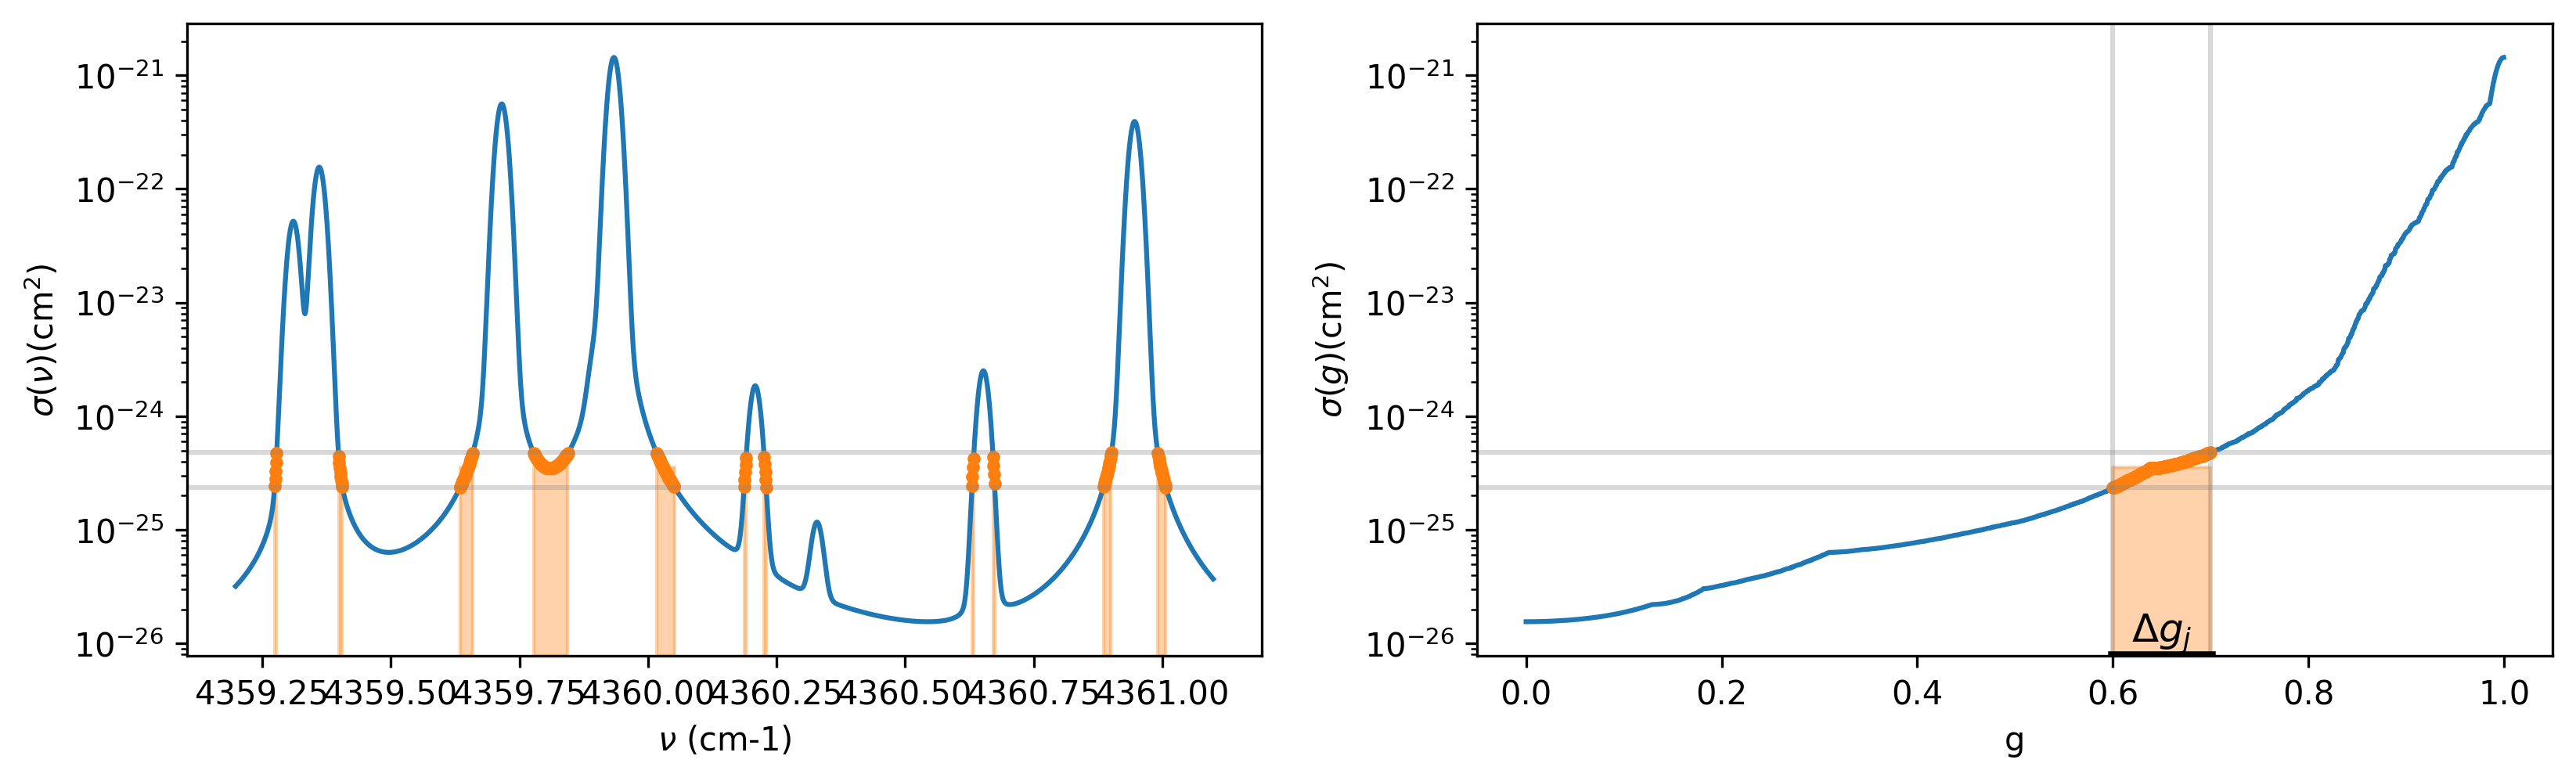
\includegraphics[width=1.0\linewidth]{fig/ckd/corrk_test.png}
    \caption{左:水の断面積を波数空間で示したもの。右:同じ断面積を$g$空間で示したもの。オレンジの領域は$g$空間の$g=0.6-0.7$に属する領域($\Delta g_i$)に含まれる断面積を示している。}
    \label{fig:ckd_fig1}
\end{figure*}


断面積$\sigma(\nu)$(もしくはオパシティ)は、ライン幅より広い波数領域でみると非単射関数、すなわち同じ$\sigma^\prime = \sigma (\nu)$の値をとる$\nu$が複数個存在する(図\ref{fig:ckd_fig1}左)。波長域が広がるにつれ非単射性が増してくる。そこで$\nu$ではなく$\sigma$の値に基づいて情報を記述することが考えられる。たとえば$\sigma(\nu)$の非負値関数である$f(\sigma(\nu)) \geq 0$をある波数幅で積分することを考える。これはリーマン積分では
\begin{align}
 I &= \int_\mathrm{min}^\mathrm{max} f(\sigma(\nu)) d \nu \approx  \sum_i f(\sigma(\nu_i)) \Delta \nu_i
\end{align}
のように、定義域$\nu$方向に分割をして足し合わせる。しかし、非単射性が増してくると、何度も同じような$\sigma$の値について和を取らないとならない。そこで値域の測度に注目して積分を行うことを考える。
いま、値域を互いに重ならない集合に分割する。たとえば$\sigma = \sigma_j$を含む微小領域$\Delta \sigma$内の値域をもつ定義域$\nu$の集合を$A_j$とすると
値域は
\begin{align}
    V = \bigcup_{j=0}^{n} A_j
\end{align}
と表すことができる。集合$A$に関する特性関数
\begin{align}
   \chi_A (\nu) &= \begin{cases}
  1, & \text{if } \nu \in A \\
  0, & \text{if } \nu \notin A
\end{cases}
\end{align}
を用いて、(非負値)単関数
\begin{align}
    s(\nu) = \sum_j^n f_j \chi_{A_j}(\nu)
\end{align}
を考える。ただし $0 \leq f_0 < f_1 < \cdots < f_n$とする。 ルベーグ積分は、集合$A_j$の測度を$m_d (A_j)$としたとき
\begin{align}
    \int_V s(\nu) d \nu = \sum_{j=0}^n f_j \, m_d (A_j)
\end{align}
と定義される。この考えを利用して、積分を行うことを考える。値域の集合として、値域を最小値から最大値までをビニングして、下から順に$j=0,1,\cdots$とする。またそれぞれの集合の代表値を$\sigma_j$とする。$f(\sigma(\nu))$を単関数で
\begin{align}
    f(\sigma(\nu)) \approx s(\nu) = \sum_j^n f(\sigma_j) \chi_{A_j}(\nu)
\end{align}
のように近似することで、
\begin{align}
 \int_V f(\sigma(\nu)) d \nu &\approx \int_V s(\nu) d \nu = \sum_j f(\sigma_j) \Delta m_j \\
 &= (\nu_\mathrm{max} - \nu_\mathrm{min}) \sum_j f(\sigma_j) \Delta g_j 
\end{align}
となる。ここに各集合の測度を$\Delta m_j = (\nu_\mathrm{max} - \nu_\mathrm{min}) \Delta g_j$とおいた。
この最後の式は、(リーマン)積分
\begin{align}
(\nu_\mathrm{max} - \nu_\mathrm{min}) \int_0^1 f(\sigma(g)) dg 
\end{align}
の近似とみることができる。また集合を無限に細かくすれば両者は一致し、
\begin{align}
\label{eq:Lebesgue}
\int_V f(\sigma(\nu)) d \nu = (\nu_\mathrm{max} - \nu_\mathrm{min}) \int_0^1 f(\sigma(g)) dg 
\end{align}
となる。

この$\sigma_j$は値域の小さいほうからビンをとっていて、$\Delta m_j$はこのビンに対応する定義域の測度、つまり定義域の対応する$\nu$空間の長さを表すものであるので、実務的には、$\sigma(g)$は $\sigma(\nu)$を細かく分割したテーブルをソートして、0-1に規格化すれば得られる。図\ref{fig:ckd_fig1}右はそのようにして得られた$\sigma(g)$である。いいかえると$\sigma$の累積分布関数である。ソートであるので単調増加関数となっている。ところでk分布という名前は、この分布関数をopacity ($k$であらわすことが多い)を用いていることに由来していると思われる。

図\ref{fig:ckd_fig1}の塗りつぶし領域は、$f (\sigma) = \sigma$ととった場合の$\Delta g_j$からの寄与を$\nu-f$空間(左)で$g-f$空間(右)で図示したものとなっている。左図で測度$\Delta m_j$は、$\nu$軸で塗りつぶしが被っている領域の和である。これを$(\nu_\mathrm{max} - \nu_\mathrm{min})$で割ったものが右図の$\Delta g_j$に対応する。

$\sigma(g)$がこのようにソートで得られたら、式(\ref{eq:Lebesgue})右辺の評価は通常の数値積分法を利用できる。たとえば、Gauss-Legendre Quadratureなどが用いられる。


\begin{figure*}[!h]
    \centering
    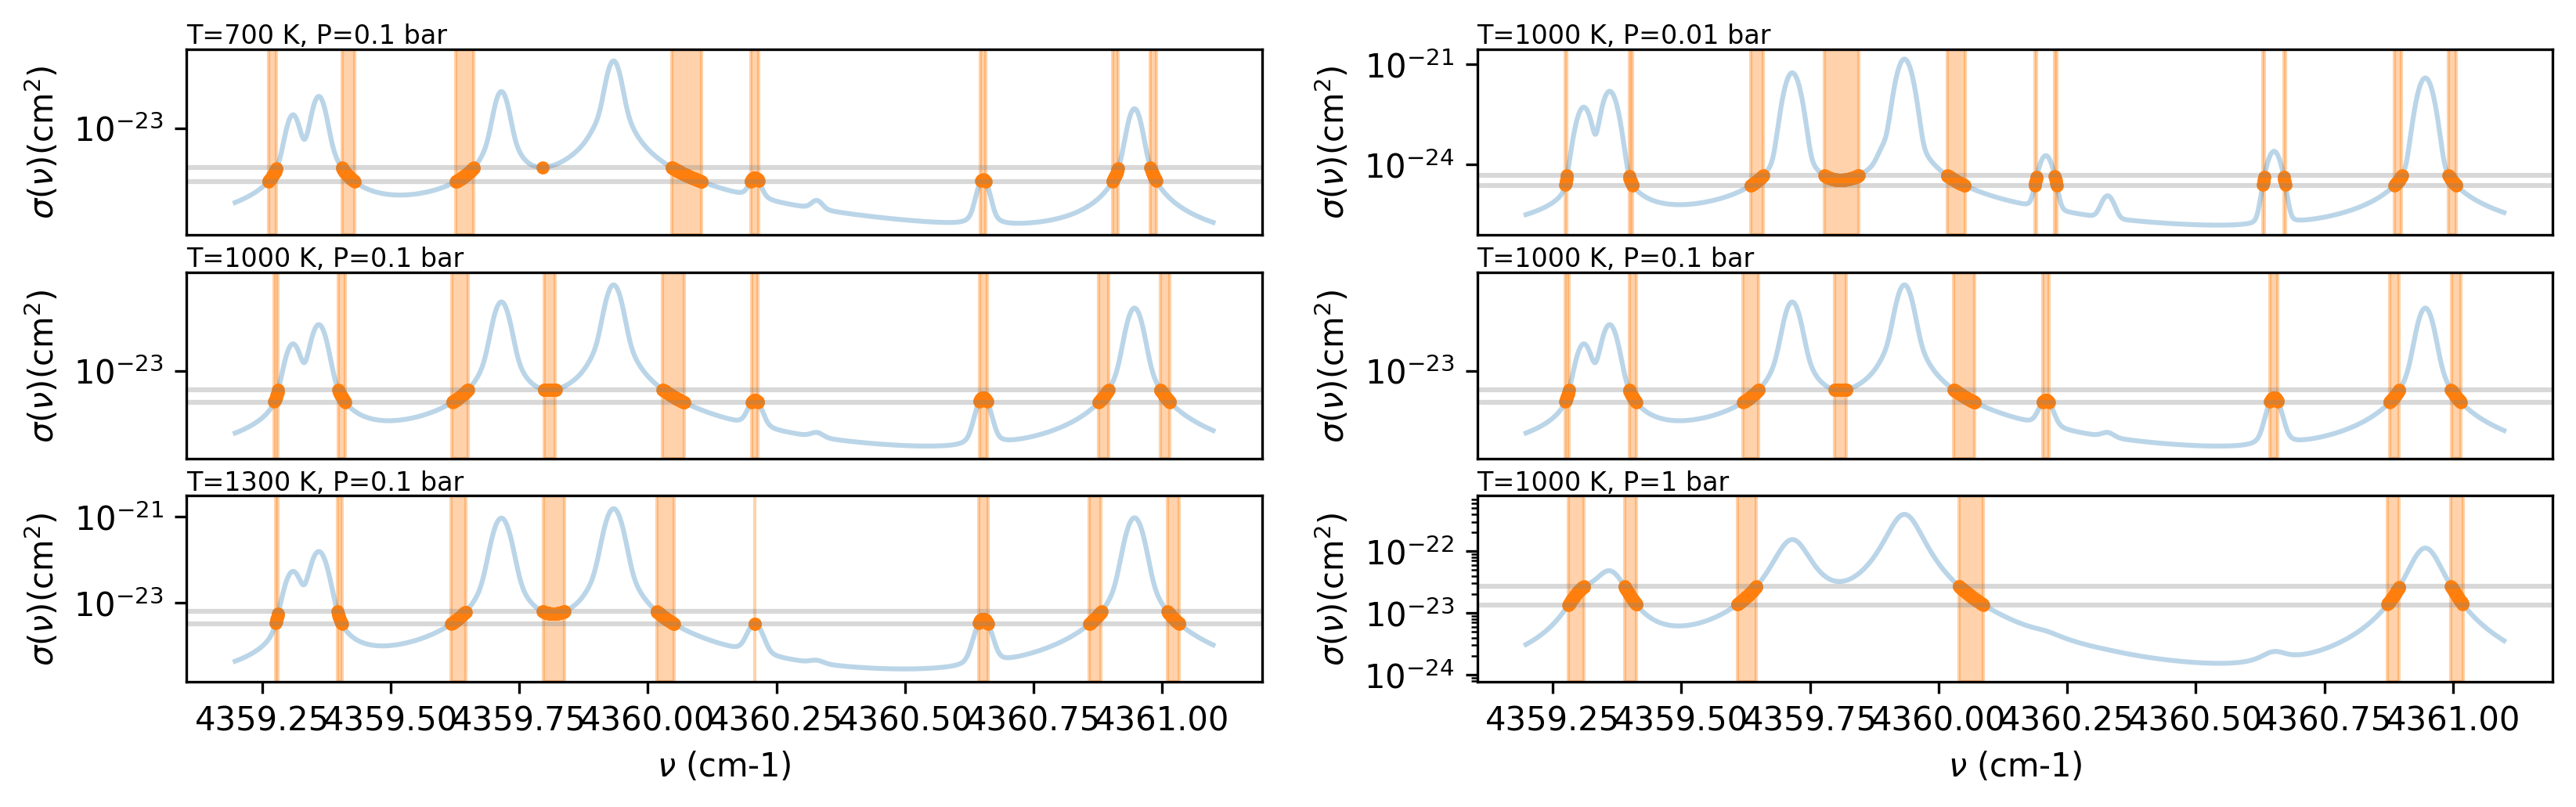
\includegraphics[width=1.0\linewidth]{fig/ckd/corrk_corr.png}
    \caption{左:圧力0.1barで温度を700,1000,1300Kと変えたときに$g$空間の$g=0.6-0.7$に属する領域($\Delta g_i$)に属する断面積をオレンジで示した。この$\delta g_i$は図\ref{fig:ckd_fig1}と同じものを採用している。 右:温度を1000Kに固定し、圧力を0.01,0.1,1barと変更した場合の$\Delta g_i$に属する断面積をオレンジでしめした。}
    \label{fig:ckd_fig2}
\end{figure*}

上では一層の積分を考えたが、放射伝達では各層ごとにオパシティがことなり、これを波数方向で積分する。これを集合$\Delta g_j$ごとの積分に置き換えることができれば、非単射性の強い状況では計算量の削減が期待できる。いいかえると図(\ref{eq:Lebesgue})左のオレンジの部分は、同程度のオパシティとしてまとめて放射伝達を解くことができる。しかしこのためには、各層で$\Delta g_j$に対応する$\nu$の集合が常に一致しないとならない。このような仮定は共単調性(comonotonicity)とよばれ、値域($\sigma$)の順序で並べたときの$\nu$の順序が常に一致していれば、$\Delta g_j$の取り方に寄らず成り立つ。相関k分布法の相関とはこのように層間の共単調性相関を仮定している。これはコピュラではフレシェ・ヘフディング上界を仮定しているのと等しい。

図\ref{fig:ckd_fig2}に温度・圧力を変えたときの$\Delta g_j$を図示する。この例で見るようにラインの中心に関してはだいたい集合が一致しているが、裾になると一致度が悪い。












